%%%%%%%%%%%%%%%%%%%%%%%%%%%%%%%%%%%%%%%%%%%%%%%%%%%%%%%%%%%%%%%%%%%%%%%%%%%%%%%%%%%%%
%																					%
%	TRABAJO: Paper Mejoras en el procesador de Redes de Petri						%
%																					%
%		Titulo: 	Soft Core parametrizable con procesamiento de Redes de Petri	%
%																					%
%		Autores:	Julian Nonino													%
%					Carlos Renzo Pisetta											%
%					Orlando Micolini												%
%																					%
%	Seccion: Marco Te�rico															%	
%	Archivo: marco_teorico.tex														%
%																					%
%%%%%%%%%%%%%%%%%%%%%%%%%%%%%%%%%%%%%%%%%%%%%%%%%%%%%%%%%%%%%%%%%%%%%%%%%%%%%%%%%%%%%

\section{Marco Teorico}
	
	\subsection{Redes de Petri}
 		
 		Una Red de Petri o Petri Net es un modelo gr�fico, formal y abstracto �til para 
 		describir y analizar el flujo de informaci�n.
 		Conforma una herramienta matem�tica aplicable, especialmente, a los sistemas 
 		paralelos que requieran simulaci�n y modelado de la concurrencia en los recursos 
 		compartidos. Existen trabajos previos donde se ha demostrado que es posible implementar 
 		sus formalismos en hardware \cite{paillertejeda}\cite{galliapereyra}

		Las Redes de Petri constan de cuatro componentes fundamentales.Fig\ref{PN}

		\begin{itemize}
			\item Plazas: Permiten representar el estado del sistema. 
    			Podr�an definirse como variables de estado que toman valores enteros (cantidad de 
    			tokens). Se representan con un c�rculo.
			\item Transiciones: Representan el conjunto de sucesos que hacen que el estado del sistema 
				cambie. Son representadas con un rect�ngulo.
			\item Arcos: Los arcos indican las conexiones entre lugares y transiciones. Nunca unen 
				dos lugares o dos transiciones en forma sucesiva. Pueden entrar o salir varios arcos 
				de una misma transici�n o de un mismo lugar. Los arcos tienen asociado un ``peso'' 
				que indica la cantidad de tokens que se consumen o generan al atravesarlo. El disparo 
				de una transici�n retira tantos tokens de cada uno de sus lugares de entrada como lo 
				indican los pesos de los arcos conectores y a�ade los tokens a sus lugares de salida 
				como lo indican los pesos de los arcos de salida.
			\item Tokens: Los tokens representan el valor espec�fico de la condici�n o estado. Son 
				graficados como un punto negro o un n�mero natural o cero dentro de una plaza.
		\end{itemize}

		\begin{figure}[h]
			\centering
			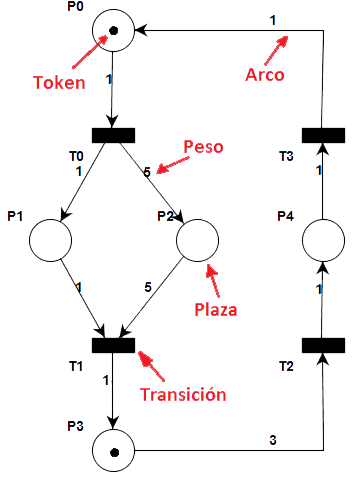
\includegraphics[width=2.5in]{RedPetri.png}
			\caption{Red de Petri}
			\label{PN}
		\end{figure}
 
		\subsubsection{Estructura de una Red de Petri}
		
			Una Red de Petri Marcada queda definida como una 5-tupla de la siguiente manera:

			\begin{center}
				$PN = \{P, T, I^-, I^+, m_0\}$ 
			\end{center}

			Donde:
			\begin{itemize}
				\item $\boldsymbol{P = \{p_1, p_2, p_3 \ldots p_m\}}$, conjunto de $m$ lugares con 
					$m$ finito y distinto de cero.			
				\item $\boldsymbol{T = \{t_1, t_2, t_3 \ldots t_n\}}$, conjunto de $n$ transiciones 
					con $n$ finito y distinto de cero.
				\item $\boldsymbol{I}$, matriz de incidencia. Esta matriz es de dimensiones $m�n$, 
					y representa los pesos de los arcos, siendo sus valores positivos cuando el arco 
					va desde una transici�n hacia una plaza; y negativos, los inversos. As� mismo, 
					para representar la estructura, esta matriz de incidencia debe separarse en dos:
					\begin{itemize}
						\item $\boldsymbol {I-}$, matriz de incidencia negativa. Esta matriz es de 
							dimensiones $m�n$ representa los pesos de los arcos que ingresan desde 
							los lugares de P a las transiciones de T.
						\item $\boldsymbol {I+}$, matriz de incidencia positiva. Esta matriz es de 
							dimensiones $m�n$ representa los pesos de los arcos que salen desde las 
							transiciones de T hacia los lugares de P.
					\end{itemize}
				\item $\boldsymbol {m_0}$ es el marcado inicial de la red, un vector de asignaci�n 
					de tokens a las plazas de la red, de esta forma se define la configuraci�n inicial 
					de los tokens de la red. Por ejemplo, puede definirse el marcado de una plaza como 
					$m(i)$, lo que indica la cantidad de tokens ubicados en la plaza ``$i$''.
					\newline
			\end{itemize}

		\subsubsection{Ejecuci�n de una Red de Petri}

			El comportamiento din�mico de una Red de Petri esta definido por la sensibilizaci�n y el 
			disparo de sus transiciones.
			\newline
			\begin{itemize}
  				\item Transici�n sensibilizada: Se dice que una transici�n $t_j$ est� sensibilizada 
  					si y solo si todas las plazas de entrada a la transici�n tienen una cantidad de 
  					tokens igual o mayor al peso indicado por el arco que la une con la transici�n. 
  					Formalmente:\newline
  				\item Disparo de una transici�n: El disparo de una transici�n es lo que provoca que 
  				el estado (marcado) de una Red de Petri cambie.
  				\newline 
			\end{itemize}

		\subsubsection{Ecuaci�n de estado de una Red de Petri}
 
			La ecuaci�n de estado determina el estado de la Red de Petri a cada instante, queda definida 
			a partir de la matriz de incidencia y un vector de disparo que indica la transici�n o 
			transiciones que deben ser disparadas.\newline
			\begin{center}$m_{k+1}=m_k+I�\delta_k$\end{center}
			Donde $m_{k+1}$ es el marcado futuro.  
		\newline
		\subsubsection{Plazas Acotadas}
		
			Un lugar $p_i$ se dice que es acotado si existe un n�mero  $k\in \mathbb{N}$ tal que, para 
			todo el conjunto de marcados alcanzables desde $m_0$, el n�mero de marcas en $p_i$ no es 
			m�s grande que k ($p_i$ se dice que es $k$-acotado). De esta manera una transici�n ademas 
			de lo visto anteriormente, debe cumplir que ninguna plaza de salida supere su cota maxima 
			$k$ luego de darse el disparo. De ser superado con un determinado disparo, este no se puede 
			llevar a cabo.
